\documentclass[twocolumn]{openjournal}

\usepackage{graphicx}
\usepackage{latexsym,amssymb}
\usepackage{amsmath,morefloats}
\usepackage[backref,breaklinks,colorlinks,citecolor=blue]{hyperref}
\usepackage{natbib,graphicx,amsmath,color,xcolor}
\usepackage{verbatim}
\usepackage{threeparttable}
\usepackage{xspace}
\usepackage{lmodern}
\usepackage{slantsc}

\newcommand{\ess}[1]{\textcolor{red}{[ESS: \bf #1]}\xspace}
\newcommand{\mrb}[1]{\textcolor{purple}{[MRB: \bf #1]}\xspace}
\newcommand{\jz}[1]{\textcolor{blue}{[JZ: \bf #1]}\xspace}

\newcommand{\mdet}{\textsc{metadetection}\@\xspace}
\newcommand{\mcal}{\textsc{metacalibration}\@\xspace}
\newcommand{\noshear}{\texttt{noshear}\@\xspace}
\newcommand{\galsim}{\textsc{galsim}\@\xspace}
\newcommand{\descwl}{\textsc{WeakLensingDeblending}\@\xspace}
\newcommand{\cosmodctwo}{\textsc{CosmoDC2}\@\xspace}
\newcommand{\buzzard}{\textsc{Buzzard}\@\xspace}
\newcommand{\ngmix}{\textsc{ngmix}\@\xspace}
\newcommand{\sep}{\textsc{sep}\@\xspace}

\xspaceaddexceptions{+}

\shorttitle{Deep-field Metacalibration}
\shortauthors{Zhang, Becker, \& Sheldon}

\begin{document}
\title{Deep-field Metacalibration}

\author{Zhuoqi (Jackie) Zhang}
\affil{Department of Astronomy and Astrophysics, University of Chicago, Chicago, IL 60637, USA}
\author{Matthew R. Becker}
\affil{High Energy Physics Division, Argonne National Laboratory, Lemont, IL 60439, USA}
\author{Erin S. Sheldon}
\affil{Brookhaven National Laboratory, Bldg 510, Upton, New York 11973, USA}


\begin{abstract}

    We introduce \textit{deep-field \textsc{metacalibration}}, a new technique
    that reduces the pixel noise in \mcal estimators of weak lensing shear
    signals by taking advantage of a smaller, deeper imaging survey for
    calibration. In standard \mcal, a small artificial shear is applied to the
    observed images of galaxies in order to estimate the response of the
    object's shape to shear, which is used to calibrate the shear estimates.
    As part of a correction for the effect of shearing the noise, extra noise
    is added to the images that increases the uncertainty on statistical shear
    estimates by $\sim 20$\%.  Our new deep-field \mcal technique leverages a
    separate, deeper imaging survey to calculate calibrations with less
    degradation in image noise.  We demonstrate that weak lensing shear
    measurement with deep-field \mcal is unbiased up to second-order shear
    effects.  We provide algorithms to apply this technique to imaging surveys,
    and describe how to generalize it to shear estimators that rely explicitly
    on object detection (e.g., \mdet).   For the Vera C. Rubin Observatory
    Legacy Survey of Space and Time (LSST), the improvement in weak lensing
    precision will depend on the somewhat unknown details of the LSST Deep
    Drilling Field (DDF) observations in terms of area and depth, the relative
    point-spread function properties of the DDF and main LSST surveys, and the
    relative contribution of pixel noise versus intrinsic shape noise to the
    total shape noise in the survey. We conservatively estimate that the
    degradation in precision is reduced from 20\% for \mcal to $<5$\% for
    deep-field \mcal, which we attribute primarily to to the increased source
    density and reduced pixel noise contributions to the overall shape noise.
    Finally, we show that the technique is robust to sample variance in the
    LSST deep fields due to their large area, with the equivalent calibration
    error being $\lesssim0.1\%$. The deep-field \mcal technique provides higher
    signal-to-noise weak lensing measurements while still meeting the stringent
    systematic error requirements of future surveys.

% We further show that for a typical lensing source,
% deep-field \mcal will decrease \mcal image pixel noise by up to $\approx30\%$, resulting
% in corresponding increases in the signal-to-noise of these sources and reductions in
% measurement errors.

\end{abstract}


\section{Introduction}\label{sec:intro}

Modern surveys that aim to measure weak lensing signals will constrain a wealth of
fundamental physics, but must meet stringent requirements on the control of systematic
effects (see, e.g., \citeauthor{MandelbaumReview}~\citeyear{MandelbaumReview} for a
review). One of the most daunting issues has been accurately measuring weak
gravitational lensing shears from survey data. For the Vera C. Rubin Observatory Legacy
Survey of Space and Time (LSST), these signals must be measured to about one part per
thousand in order to not dominate the overall error budget and degrade cosmological
constraints \citep{huterer2006,descsrd}. A large number of systematic effects and
measurement biases must be overcome to reach this goal, including correcting for the
point-spread function (PSF), noise biases, model biases, selection effects, blending
effects, and detection effects (see, e.g.,
\citeauthor{MandelbaumReview}~\citeyear{MandelbaumReview} for a comprehensive discussion
and references). So far, the community has developed three techniques
that can reach the part-per-thousand accuracy required by LSST without direct
calibration from image simulations. These techniques are BFD \citep{BernBFD2016,ba14},
FPFS \citep{li2018fpfs,li2022fpfs}, and \mcal \citep{SheldonMcal2017,HuffMcal2017},
all of which meet LSST requirements for unblended, isolated sources. The newly
introduced \mdet technique promises to reach part-per-thousand accuracy even in the
presence of object detection and blending \citep{SheldonMdet2022}, but much work
remains to fully realize the potential of this technique in realistic survey scenarios.

Despite their success, the \mcal and \mdet techniques as currently implemented
have a nontrivial drawback. In order to reach the required accuracy in shear
measurement, they effectively double the pixel noise variance in the survey
images or equivalently reduce the signal-to-noise of every source by
approximately a factor of $1/\sqrt{2}\approx30\%$. As described below, this
effect comes from a numerical correction needed to account for sheared pixel
noise in the \mcal pipeline. This feature results in a loss of precision in the
final cosmological analysis at the $\sim 20\%$ level \citep{SheldonMcal2017}.

Interestingly, modern surveys typically have a wide-field imaging campaign, which forms
the survey used for weak lensing shear measurements, and a deep-field imaging campaign,
which is a much smaller region that is surveyed longer, eventually reaching depths of
$10\times$ or more than the main wide-field survey. See for example the Dark Energy
Survey deep-fields work \citep{DESDeepFields} or the planned LSST Deep Drilling Fields
(DDFs) \citep{lsst-ddf-design,lsst-ddf-depth,ivezic2019lsst}. Although \mcal currently
does not take advantage of deep-field data, the BFD estimator explicitly uses it,
avoiding increases in the wide-field image pixel noise in the analysis.

In this work, we propose a new technique, \textit{deep-field \textsc{metacalibration}},
which greatly reduces noise degradation by taking advantage of a
deep-field survey to derive calibrations. The standard \mcal estimator for
a mean shear has two
components, the uncalibrated shape measurements $\langle \mathbf{g} \rangle$ and the
mean \mcal response matrix $\langle\mathbf{R}\rangle$, both of which are computed from
the wide-field survey data. These quantities are combined to form the final shear
estimate as
\citep{HuffMcal2017,SheldonMcal2017}
\begin{equation*}
\hat\gamma \equiv \langle\mathbf{R}\rangle^{-1}\langle \mathbf{g} \rangle\ .
\end{equation*}
The deep-field \mcal estimator works by computing the mean \mcal response matrix
$\langle\mathbf{R}\rangle$ from the deep-field survey data instead of the wide-field
survey data. We show below that with this change, we can carefully arrange the
deep-field \mcal estimator to double the effective pixel noise variance in the
deep-field survey data only. Since the deep-field survey data is lower-noise than the
wide-field survey data in the first place, the final deep-field \mcal estimator achieves
higher precision than the original \mcal technique. We find that in all cases this
estimator is as accurate as the original \mcal estimator, achieving better than
part-per-thousand accuracy in the overall shear measurement. We demonstrate that with
this new technique, we will decrease the pixel noise in \mcal images by $\approx30\%$,
increase the signal-to-noise of \mcal weak lensing sources and decreasing their shape noise.
The exact change in the pixel noise depends in detail on the relative depth and PSF
distributions of the wide- and deep-field surveys. We further estimate an at least
$\approx15\%$ increase in the statistical precision of weak lensing analyses with
Rubin LSST due to the decreased pixel noise. We conservatively estimate that the
uncertainty in the shear estimator
is degraded by $<5\%$ rather than the approximately 20\% degradation in
standard \mcal.

The primary concern when utilizing only the deep-field data to compute the \mcal
response is sample variance. The deep-field survey typically covers a much smaller
area of the sky than the wide-field survey. The \mcal response depends on the properties
of the galaxies from which it is computed (e.g., their profiles, sizes, etc.) and so
will inherit sample variance in those properties due to large-scale structure. We
estimate this effect with two complementary mock catalogs, finding that for the large
$\approx35$ deg$^2$ area of the LSST DDFs \citep{lsst-ddf-design,ivezic2019lsst}, the
resulting sample variance scatter in the \mcal response will be in the range of 0.05\%
to 0.1\%. This level meets LSST requirements, and extensions of our technique that
reweight the deep-field galaxy populations to match the wide-field ones may reduce this
sample variance further.

Our paper is organized as follows. In Section~\ref{sec:math}, we review standard \mcal
and introduce the formalism for deep-field \mcal. Then in Section~\ref{sec:results}, we
cover the main results of our work, including tests of shear calibration (\ref{sec:mc})
and estimates of the gains in signal-to-noise (\ref{sec:sizedepth}). In
Section~\ref{sec:terms}, we present a discussion of the relative importance of various
corrections in the deep-field \mcal estimator. We address the issue of sample variance
in the deep-fields in Section~\ref{sec:sv}. Finally in Section~\ref{sec:conc}, we
summarize our results and suggest avenues for further research.

\section{Deep-field \mcal Formalism}\label{sec:math}

In this section, we introduce the underlying algorithms of deep-field \mcal and describe
one method to apply those algorithms to a realistic survey composed of wide- and
deep-field imaging datasets. We start by examining standard \mcal images in our
formalism. We then use the intuition developed there to motivate correction terms that
can be applied to the deep-field and wide-field images to enable shear measurement.
Finally, we specify the details of how we combine the deep- and wide-field image sets in
practice, including how to make selections on the sources and compute the deep-field
\mcal response.

For conciseness, we adopt the following notation. We denote a convolution
operation of two images as $I_1 \star I_2$, deconvolution as $I_1/I_2$,
and pointwise addition or subtraction as $I_1\pm I_2$. We also define two special
operators on images. First, we define a shearing operator $Y[I, \gamma]$ that shears
the image $I$ by the shear $\gamma$. Second, we define a \mcal operator,
$M[I, N, P, P_r]$, defined as
\ess{should we move this to the later section?}
\mrb{IMHO, no. I added a reference to the relevant section where it is derived.}
\begin{eqnarray} \label{eq:mcalop}
\lefteqn{M[I, N, P, P_r, \gamma]=} & & \\\nonumber
& &\ \ Y[I/P, \gamma] \star P_r + Y[N/P, -\gamma] \star P_r
\end{eqnarray}
where $I$ is an image, $N$ is a second image (usually pure noise), $P$ is the image PSF,
$P_r$ is the \mcal reconvolution PSF, and $\gamma$ is a shear. This operator performs
the standard steps of the \mcal algorithm, including the correction for sheared noise as
described in \citet{SheldonMcal2017}. We present a detailed description and derivation
of this operator below in Section~\ref{sec:mcalagain}. We have not specified the exact
numerical implementation of these operators for pixelated images. In practice, we rely
on the \galsim package which provides high-quality, performant implementations
\citep{GALSIM2015}. Depending on the context, these implementations rely on fast-Fourier
transforms and interpolations of various kinds and orders. Our implementation is
publicly available.\footnote{\url{https://github.com/beckermr/deep-metacal}}

In what follows, we work with single images for both the wide and deep surveys.
Modern surveys use a strategy of tiling the sky with overlapping images taken
at different epochs.  Multi-epoch data can be handled by forming postage stamp
coadds around each object \citep{psc} or for \mdet, by using coadds without PSF
discontinuities \citep{BeckerMdet2022,SheldonMdet2022}. These data products
have well defined PSFs, and the coadd noise properties can be determined by
running pure noise images through the coaddition process. The algorithms below
generalize to these multi-epoch scenarios.

\subsection{Standard \mcal}

The standard \mcal estimator is based on a linear expansion of the shape of an object,
$\mathbf{e}$, in the true $\gamma$,
\begin{eqnarray}
\mathbf{e} & = & \left. \mathbf{e} \right|_{\gamma=0}
+ \left.\frac{\partial\mathbf{e}}{\partial\gamma}\right|_{\gamma=0} \gamma
+ {\cal O}(\gamma^2)\nonumber\\
& \equiv & \left. \mathbf{e} \right|_{\gamma=0}
+ \mathbf{R} \gamma
+ {\cal O}(\gamma^2)\nonumber
\end{eqnarray}
where we have defined the response matrix $\mathbf{R}$ as
\begin{equation}
R_{ij} \equiv \left.\frac{\partial e_i}{\partial\gamma_j}\right|_{\gamma_j=0}\ .
\end{equation}
Under the assumption that the intrinsic shapes of objects average to zero,
$\langle \left. \mathbf{e} \right|_{\gamma=0} \rangle = 0$, then we get to linear order
\begin{equation*}
\langle\mathbf{e}\rangle \approx \langle \mathbf{R} \gamma\rangle,
\end{equation*}
% \langle\mathbf{e}\rangle = \langle \mathbf{R} \rangle \langle\gamma\rangle
which demonstrates that true shear is weighted by the response
in the mean ellipticity.  We can then calculate the response weighted mean shear
\begin{equation*}
    \hat{\gamma} \equiv \langle \mathbf{R} \rangle^{-1} \langle \mathbf{e} \rangle \approx \langle \mathbf{R} \rangle^{-1} \langle \mathbf{R \gamma} \rangle.
\end{equation*}

In standard \mcal the mean response $\langle \mathbf{R} \rangle$ is computed by applying
small artificial shears to the observed images of objects and using a finite difference
derivative to measure how their shapes change. Including the shape measurements where no
shear has been applied, this process generates five shape measurements per object. These
are the one with no shear, which we denote as \texttt{noshear},
$\pm\epsilon_1$ which we denote \texttt{1p} and \texttt{1m}, and
$\pm\epsilon_2$ which we denote \texttt{2p} and \texttt{2m}.
A numerical response per object can be constructed via
\begin{equation*}
R_{ij} \approx \frac{e_i^{+j} - e_i^{-j}}{2\epsilon}\ .
\end{equation*}
where we have denoted the shape measurement as $e_i^{\pm j}$ for the $i$th shear
component with  with applied shear $\pm\epsilon_j$ on the $j$th axis. The responses per
object are typically quite noisy and so the recommended estimator for the mean shear of
a region of the sky averages the response and shapes separately as above so that
\begin{equation*}
\langle R_{ij} \rangle = \frac{\langle e_i^{+j} \rangle - \langle e_i^{-j} \rangle}{2\epsilon}\ .
\end{equation*}
The averages $\langle\ \rangle$ above are taken over each of the five shapes above
separately after all selections have been applied in order to correct for selection
effects. That is, we aggregate the shape measurements from all of the \noshear images,
all of the \texttt{1p} images, etc. into five separate catalogs, apply the object
selections to those catalogs separately, compute the average shape over those catalogs
separately, and then finally compute the mean shear and response from those averaged
shears. This procedure is the one described in \citet{SheldonMdet2020} for \mdet but
applies equally well to \mcal. However, one can use separate shear and selection
responses with a single set of selections as done in \citet{SheldonMcal2017}. When
applied to isolated objects, this technique can achieve the part-per-thousand accuracy
required by LSST \citep{HuffMcal2017,SheldonMcal2017}.

The numerical implementation of standard \mcal has two key features which are relevant
to the discussion of deep-field \mcal below. First, as discussed in
\citet{SheldonMcal2017}, one must correct for the effects of sheared background noise
when estimating the response to shear via finite differencing. When applying an
artificial shear to a noisy image, the sheared background noise becomes correlated
across adjacent pixels. This effect, if left uncorrected, biases the shape measurements
for the response images \texttt{1p}, \texttt{1m}, etc. relative to those from the
\noshear images, producing a biased shear estimator. \citet{SheldonMcal2017} tried a
variety of schemes to correct for this effect, but settled on the following procedure.
Before shape measurement under an artificial shear $\epsilon_j$, a pure noise image with
the same noise spectrum as the original image is rotated by 90 degrees, sheared by
$\epsilon_j$, rotated back, and then added to the sheared original image. As detailed
below, this procedure cancels the biases in the shape measurements but has the net
effect of effectively doubling the pixel noise variance in the image. It is this
inefficiency we are seeking to rectify in this work. Second, in order to artificially
shear an image, one must first deconvolve the PSF. This procedure is most easily done in
Fourier space where it is a simple division. However, numerical instabilities can arise
since one ends up dividing by small numbers at Fourier modes where the original PSF is
nearly zero. To rectify this, one typically reconvolves the image with a slightly larger
PSF, called the \textit{reconvolution PSF}, which controls these numerical instabilities
by suppressing the affected Fourier modes.


\subsection{Standard \mcal Revisited}\label{sec:mcalagain}

In order to gain insight into the deep-field \mcal algorithms below, let's consider the
standard \mcal algorithm in our notation. For this, let's denote the galaxy as $G$, the
PSF as $P$, our noise field as $N$, and the \mcal reconvolution PSF as $P_r$. In this
notation, the observed image of an object is $I = G\star P + N$. That is, we convolve
the galaxy $G$ with the PSF $P$, $G\star P$, and then get a noisy realization of the
noiseless image, $G\star P + N$.

In \mcal, we want an image of the object $G$, but with a small shear $\epsilon$ applied.
A shape measurement of this image of the object will be used to compute the response
$\mathbf{R}$ above. For now let's consider a small positive shear $\epsilon$
(The exact direction doesn't matter so we will drop the typical $1,2$
subscripts.) We need to deconvolve the PSF (i.e. $I/P$) before applying this small
shear, so we get for our image $I$
\begin{equation} \label{eq:yop}
Y[I/P,\epsilon].
\end{equation}
This process has two effects. First, the deconvolution amplifies the noise in the
image. This happens since in Fourier space, where this operation is a division, $P$ is
close to zero for Fourier modes whose wavelengths are much smaller than the size of the
PSF. Dividing by these small numbers amplifies noise at high-frequency modes. Second,
the amplified noise, which no longer has a flat power spectrum, is sheared, resulting
in an anisotropic noise power spectrum, even if the original PSF were round.

Note that deconvolution and shearing commute with addition, so we can write equation
\ref{eq:yop} as
\begin{equation*}
Y[I/P,\epsilon] = Y[(G+N)/P,\epsilon] = Y[G/P,\epsilon] + Y[N/P,\epsilon]
\end{equation*}
To suppress the amplified noise at high frequency modes, we convolve the image
with a reconvolution PSF $P_r$ that is
slightly larger than the original PSF $P$ in real-space
\begin{equation*}
Y[I/P,\epsilon]\star P_r = Y[G/P,\epsilon]\star P_r + Y[N/P,\epsilon]\star P_r\ .
\end{equation*}
Note after this suppression, the noise power spectrum is still not isotropic.
To correct for this effect, \citet{SheldonMcal2017} created a compensating
noise image $N'$, with the same
noise distribution as $N$, and put through the same process as the original image $I$
above but with the opposite shear
\begin{equation*}
Y[N'/P,-\epsilon]\star P_{r}\ .
\end{equation*}
This image is added to our result above giving a total image
\begin{equation*}
Y[G, \epsilon] \star P_r + Y[N/P, \epsilon] \star P_r + Y[N'/P, -\epsilon] \star P_r\ .
\end{equation*}
The three terms in this equation are the sheared galaxy convolved by the reconvolution
PSF $P_r$, the sheared noise in the original image, $Y[N/P, \epsilon] \star P_r$, and
finally the sheared noise correction needed by \mcal, $Y[N'/P, -\epsilon] \star P_r$.
This process motivates the definition of the \mcal operator $M[I, N', P, P_r, \epsilon]$
in Equation~\ref{eq:mcalop} that does exactly these manipulations. A similar set of manipulations generates
the \noshear and $-\epsilon$ cases. In total then, we have for the \noshear,
$+\epsilon$, and $-\epsilon$ images
\begin{eqnarray}
  \lefteqn{M[I, N', P, P_r, \phantom{-}0]} & & \nonumber \\
    & &=Y[G, \phantom{-}0] \star P_r + Y[N/P, \phantom{-}0] \star P_r + Y[N'/P, \phantom{-}0] \star P_r \nonumber \\
    \lefteqn{M[I, N', P, P_r, +\epsilon]} & & \nonumber \\
      & &=Y[G, +\epsilon] \star P_r + Y[N/P, +\epsilon] \star P_r + Y[N'/P, -\epsilon] \star P_r \nonumber \\
  \lefteqn{M[I, N', P, P_r, -\epsilon]} & & \nonumber \\
    & &=Y[G, -\epsilon] \star P_r + Y[N/P, -\epsilon] \star P_r + Y[N'/P, +\epsilon] \star P_r \nonumber\ .
\end{eqnarray}

There are a few key features to notice in the various images above. First, notice that
the $+\epsilon$ image and the $-\epsilon$ have statistically identical noise
distributions due to the matched set of opposite signs on the terms like
$Y[N/P,\pm\epsilon] \star P_r$. The set of operations in the terms
$Y[N/P,\pm\epsilon] \star P_r$  will generate correlations in the noise of adjacent
pixels, the exact structure of which depends in  detail on the initial noise
distribution in $N$, the PSFs involved, and the applied shear. By adding a noise field
sheared with the opposite sign to the original artificial shear, we end up with noise
fields whose distribution arises from the set of operations
\begin{equation*}
Y[N/P, -\epsilon] \star P_r + Y[N'/P, +\epsilon] \star P_r
\end{equation*}
or
\begin{equation*}
Y[N/P, +\epsilon] \star P_r + Y[N'/P, -\epsilon] \star P_r\ .
\end{equation*}
These two images have noise realized from the same underlying distribution since
addition is commutative and terms with $+\epsilon$ are always paired with a $-\epsilon$
term. Second, notice again that the effective noise variance has been doubled relative
to original image since we have now added two realizations of the original noise field
$N$. Third and finally, notice that the noise distribution between the \noshear and the
$\pm\epsilon$ images does not match precisely. Due to this fact, at least in principle,
the noise biases on the shape measurements would not be the same, causing the \mcal
response computation to be incorrect. However, due to the opposing signs in the terms
above, these differences cancel, leaving the \mcal estimator unbiased.

Before continuing, it is worth unpacking how the cancellation of the sheared noise
biases happens.  Imagine an image where we have applied a noise field sheared by
$\pm\epsilon$ but have done nothing to correct for that shearing. Then to linear order
in the shape measurement of an object in that image we can write
\begin{equation*}
\mathbf{e}_{\pm\epsilon} = \mathbf{e}_{\epsilon=0} \pm \epsilon b
\end{equation*}
where $\mathbf{e}_{\pm\epsilon}$ is our shape measurement,
$\mathbf{e}_{\epsilon=0}$ is the result we'd get if we had not sheared the noise, and
$\pm \epsilon b$ is the bias in the shape measurement due to the shearing of the noise.
If we were to average two measurements of the object with the noise fields sheared in
opposite directions, we'd get
\begin{equation*}
\frac{\mathbf{e}_{+\epsilon} + \mathbf{e}_{-\epsilon}}{2}
= \hat{\mathbf{e}}_{\epsilon=0} + \frac{1}{2}\epsilon b - \frac{1}{2}\epsilon b
= \hat{\mathbf{e}}_{\epsilon=0}\ .
\end{equation*}
In other words, for small shears $\epsilon$, the \mcal procedure of adding in a noise
field sheared by the opposite sign shear when building the \texttt{1p}, \texttt{1m}, etc.
images cancels the differences in shape measurements under the mismatched noise fields
of the \noshear versus the \texttt{1p}, \texttt{1m}, etc. images to linear order. In
deep-field \mcal, we'll need to arrange this cancellation and matching of the \noshear
image as well, but between the wide- and deep-field images.

In deep-field \mcal, our goal is to avoid the effective doubling of the variance in the
images by taking advantage of a low-noise deep-field image set. One of course still
needs the shape measurements from the wide-field image set for cosmological inference.
We originally needed to double the variance to cancel biases due to the image
manipulations used to compute the \mcal response. If we computed the \mcal response in
the deep-field images only, then we could use the same corrections for the sheared
noise, only doubling the effective noise of the deep-field image set. We'd then expect
an increase in the signal-to-noise of a given source by
$\approx\sqrt{2\sigma^2_{\rm wide}/(\sigma^2_{\rm wide} + 2\sigma^2_{\rm deep})}$.
This factor is the effective variance for standard \mcal in the wide-field divided by
the effective variance for deep-field \mcal, the wide-field variance plus twice the
deep-field variance. For deep-field imaging sets that are $\approx10\times$ deeper than
the wide-field survey, $\sigma^{2}_{\rm deep}/\sigma^{2}_{\rm wide}\approx 1/10$, and
this factor is $\approx1.30$ or about a $\approx30\%$ increase.

In order to make use of this idea, we'll still need to satisfy the relationships between
the pixel noise distributions in the \noshear and \texttt{1m}, \texttt{1p}, etc. images
above. These properties are that the noise correlations in the images used to compute
the response match statistically between the positively and negatively sheared images,
and that the noise correlations in the \noshear image should match those used for the
response computation but with no shear applied to the image. A further constraint is
that for \mdet, we want the deep- and wide-field images to have the same PSF in order
to match the detection and blending effects between the two sets of images. We describe
how to arrange these relationships below.

\begin{figure*}
    \centering
    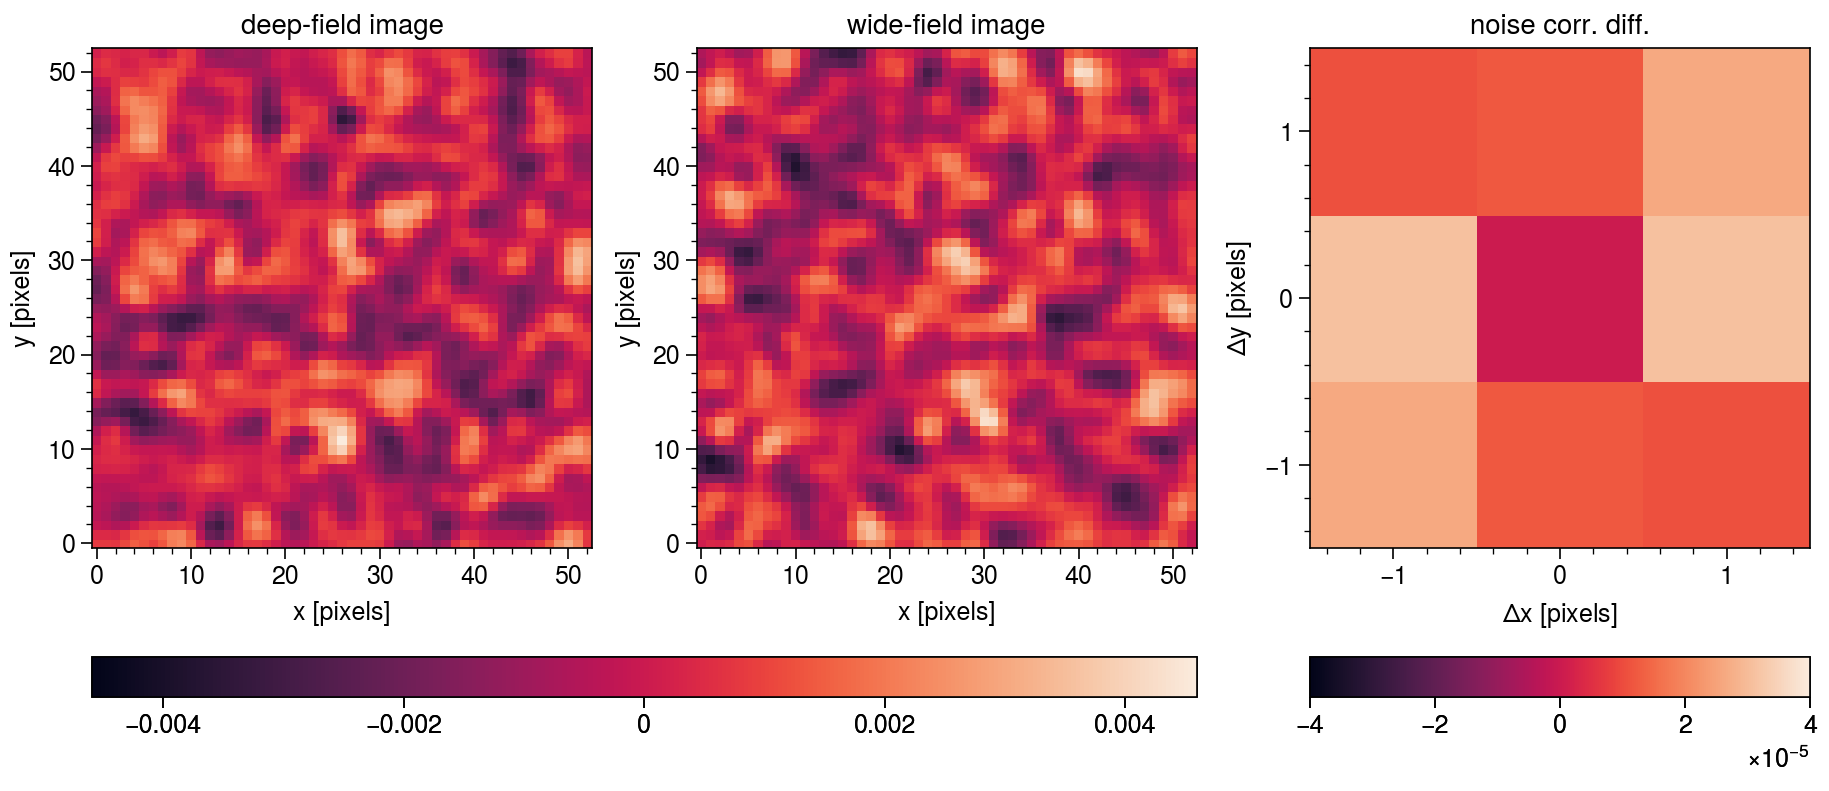
\includegraphics[width=\linewidth]{noise_corr.png}
    \caption{
      \textit{Left \& middle panel}: Example pure noise images from the deep- and wide-field image
      sets after deep-field \mcal. Visually, the two noise images exhibit the same noise correlation structure.
      \textit{Right panel}: The difference in the average pixel-pixel correlation matrix of $10^6$ deep- and
      wide-field images $\hat I_{w,d}$. The difference is of order $10^{-5}$, indicating good numerical
      performance of our codes.
    } \label{fig:pixel_correlation}
\end{figure*}


\subsection{Deep-field \mcal}\label{sec:deepmcal}

In order to proceed, let's first start with a naive setup where we run \mcal on the
deep-field images and simply match the PSF of the wide-field image to the deep-field in
the most naive way. For the wide-field image after PSF matching to deep-field
reconvolution PSF $P_{r,d}$ we get
\begin{equation*}
  \left(G\star P_{w} + N_{w}\right)/P_{w} \star P_{r,d} = G \star P_{r,d} + N_{w}/P_{w} \star P_{r,d}
\end{equation*}
and for the deep-field image after applying \mcal we get
\begin{eqnarray}
M[I_{d}, N_{d}', P_{d}, P_{r,d}, \epsilon] & = & Y[G, \epsilon] \star P_{r,d} \nonumber \\
  & & + Y[N_{d}/P_{d}, \epsilon] \star P_{r,d} \nonumber \\
  & & + Y[N'_d/P_d, -\epsilon] \star P_{r,d} \nonumber\ .
\end{eqnarray}
Here $P_{w,d}$ are the PSFs for the wide- and deep-field images, $P_{r,w/d}$ are
reconvolution PSFs for the wide- and deep-field images that are large enough to suppress
excess noise from deconvolution by $P_{w,d}$, and $N_{w,d}$ are noise images with the
wide- and deep-field noise levels. Notice that the noise in the wide-field image is
$N_{w}/P_{w} \star P_{r,d}$ while the noise in the deep-field image is $Y[N_{d}/P_{d},
\epsilon] \star P_{r,d} + Y[N'_d/P_d, -\epsilon] \star P_{r,d}$. The key idea is that
Monte Carlo realizations of images with these noise properties are computable from only
the knowledge of the PSFs and noise levels involved. In order to match
the noise properties between the wide- and deep-fields, we can simply compute a Monte
Carlo realization of the final wide-field noise and add it to the deep-field image and
vice versa. To take care of the PSF matching, we use the larger in size of the two
reconvolution PSFs, $P_{r,w/d}$. We call this PSF $P_{r}$. A nice side effect of this
choice for $P_{r}$ is that all of the PSF handling operations are now stable since by
definition $P_{r}$ is big enough to suppress noise from deconvolution by either
$P_{r,w}$ or $P_{r,d}$.

In detail then, we define the following wide- and deep-field correction images
\begin{equation}\label{eqn:cw}
C_{w}(\epsilon=0) = M[N^{''}_d, N^{'}_d, P_d, P_{r}, \epsilon=0]
\end{equation}
\begin{equation}\label{eqn:cd}
C_{d} = N'_{w}/P_{w} \star P_{r}
\end{equation}
These, stated simply, are a noise realization from the deep-field image put through
\mcal with zero applied shear and a straight-forward deconvolution and reconvolution
operation done on a noise realization from the wide-field images. The wide-field
correction image is added to a PSF-matched wide-field image and the deep-field
correction image is added to the deep-field image after standard \mcal has been applied.
The final images we use for shear estimation in \mcal are then
\begin{eqnarray}
\hat I_{w} & = & I_{w}/P_{w} \star P_{r} + C_{w}(\epsilon=0)\\
\hat I_{d} & = & M[I_{d}, N_{d}', P_{d}, P_{r}, \epsilon] + C_{d}\ .
\end{eqnarray}
Expanding these equations out we find that the noise applied to both images can be
computed as
\begin{equation*}
N_{w}/P_{w}\star P_{r} + Y[N_{d}/P_{d}, \alpha] \star P_{r} + Y[N'_d/P_d, -\alpha] \star P_{r}
\end{equation*}
with $\alpha\in\{0,+\epsilon,-\epsilon\}$. As is clear, we've avoided adding an extra
wide-field noise image at the cost of adding two extra deep-field noise realizations,
our original goal above. We've also matched the noise distributions in the images in the
same way as standard \mcal.

In detail, each term in $\hat I_{w,d}$ serves a specific purpose, correcting for a
specific effect. The term $I_{w}/P_{w} \star P_{r}$ serves to match the PSF of the
wide-field image to the \mcal reconvolution PSF. Remember that this reconvolution PSF
$P_r$ is the same for both the wide- and deep-field images. Thus this term serves to
bring the wide-field PSF to the final PSF of the deep-field image $\hat I_{d}$. The
\mcal response of a galaxy to shear depends critically on the PSF, in terms of both its
value (e.g., larger galaxies relative to the PSF respond more to shear), and through
more subtle effects like selection, blending, and detection. By matching the PSFs of the
images, we ensure that these effects are the same in both the wide- and deep-fields. The
term $C_{w}$ serves to add in noise levels and correlations from the the deep-field
image put through \mcal. Thus effects like noise bias on the shears or selections on
signal-to-noise will be the same in both the wide- and deep-field images. The term
$C_{d}$ serves a similar purpose, but for the deep-field images by adding in the noise
of a PSF-matched wide-field image. The term $M[I_{d}, N_{d}', P_{d}, P_{r}, \epsilon]$, is
standard \mcal applied to the deep-field image. It thus plays the role of standard
\mcal. More explicitly, first, it applies the counter-factual shear $\epsilon$ to the
image for computing the response. Second, it adds in the correction for sheared
correlated noise needed to get unbiased response computations. Finally, it PSF matches
the deep-field image to the reconvolution PSF $P_{r}$, ensuring again that the overall
response, selections, blending, and detection effects are the same in the wide- and
deep-fields.

In Figure~\ref{fig:pixel_correlation}, we compare the correlated noise fields for the
wide- and deep-field images, $\hat I_{w,d}$. The left and middle panels show example
realizations of the noise fields. Visually, the correlation structure is similar. To
test their agreement numerically, we compute the pixel-pixel correlation matrix for
adjacent pixels in both images, averaging over $10^6$ realizations to reduce the noise.
We show the difference between the wide- and deep-field pixel-pixel correlation matrices
in the right panel. They agree to ${\cal O}(10^{-5})$, indicating that our numerical
implementation of this technique is working well. We find similar fractional agreement
in the overall pixel variance as well.

Finally, we note that while we have chosen to PSF match the images in our derivation
above, we could have done the same derivation with $P_{r}$ replaced by $P_{r,w/d}$ for
each of the wide- and deep-field images. This set of manipulations would result in
images with statistically equivalent noise before convolution with $P_{r,w/d}$. If one
can arrange for the shape estimate to be made on the pre-PSF image, then it may be
possible avoid the PSF matching all together. We leave exploring this technique to
future work where one should also test the effect of not PSF matching on the detection
process and resulting detection and/or blending biases.

\subsection{Handling Populations of Objects in the Wide- and Deep-field Samples}\label{sec:statmatch}

While the derivation above has demonstrated how to take two images and match them
statistically for \mcal, it has not addressed how to apply this technique to a realistic
survey where there will be variations in the noise, PSF, and galaxy properties between
the wide- and deep-field image sets. In particular, we will not have a deep-field image
of every wide-field object. Thus in an actual survey, we will instead rely on the fact
that the deep-field images have a statistically representative set of objects for the
wide-field. The most obvious way in which this assumption is invalid is sample variance.
We estimate those effects in Section~\ref{sec:sv} below, demonstrating that for a Rubin
LSST-like survey, we should not be limited by this effect.

In order to actually compute a shear estimate, we propose the following processing
algorithm.
\begin{enumerate}
\item For every wide-field image
\begin{enumerate}
  \item Draw a deep-field image at random.
  \item Use the equations above to compute $\hat I_{w}$ for the \noshear
    and $\hat I_{d}$ for the $\pm\epsilon_{1,2}$ (i.e., \texttt{1p}, \texttt{1m}, etc.)
    cases.
  \item Perform shape measurements on each of the five images from the last step.
  \item Accumulate a catalog of all shape measurements separately for each of the
    five images.
\end{enumerate}
\item Apply the same set of selection cuts separately to each of the five catalogs from
  the last step.
\item Use the mean shapes of each of the five catalogs separately after selection in
  order to compute the response corrected shear via Equation~\ref{eqn:r}.
\end{enumerate}
This procedure does a brute-force Monte Carlo integral over the
distributions of the wide- and deep-field image properties by using the data itself as
random draws. The final shear estimate is obtained by computing the \mcal response from the deep-field
catalogs and the shear signal of interest from the wide-field catalog. For the mean
shear, this estimator is
\begin{eqnarray}\label{eqn:r}
\hat\gamma & = & \langle\mathbf{R}_d\rangle^{-1} \langle\mathbf{e}_{w}\rangle\\
R_{d,ij} & = & \frac{\langle e^{+\epsilon_j}_{d,i}\rangle - \langle e^{-\epsilon_j}_{d,i}\rangle}{2\epsilon}\nonumber
\end{eqnarray}
where the brackets $\langle\ \rangle$ indicate the average shape after selection,
$\mathbf{e}_{w}$ is the set of wide-field shapes, and $e^{\epsilon_j}_{d,i}$ is the set
of deep-field shapes measured  with \mcal shear $\epsilon_j$ in the $i$th shape
component. Higher-order statistics like two-point functions can be computed from
any of the common estimators \citep[see, e.g.,][for examples]{desy3shear}.

In practice, there may be several avenues for improvement on the naive brute-force
approach taken above. First, as we show below, deep-field \mcal works best when the PSF
of the deep-field images is the same size or smaller than the PSF of the wide-field
images. Thus it may be advantageous to subselect deep-field images by their PSF size
before pairing them to the wide-field images. A danger with this alternative procedure
is any potential inadvertent additional selections applied to the objects that cannot be
corrected by \mcal (because they happen before \mcal is applied). Another danger is
increasing the sample variance since now effectively only a subset of the deep-field
image set is used for each wide-field image. In practice, when coadded over hundreds or
epochs, the wide- and deep-field images in surveys like LSST will likely have very
similar, relatively narrow PSF distributions. Given that deep-field \mcal is still
effective even if the deep-field PSF is marginally bigger than the wide-field PSF, this
alternative matching procedure may only supply marginal gains.

\begin{table*}
  \centering
  \begin{threeparttable}
  \caption{Shear Calibration Results for Deep-field \mcal}
  \label{tab:shearmeas}

  \begin{tabular}{cccccc}
    \hline
    \noalign{\vskip 1mm}
    case & noise\tnote{a} & PSF\tnote{b} & galaxy\tnote{c} & m [$10^{-3}$ $3\sigma$ error] & c [$10^{-4}$ $3\sigma$ error]\\
    \noalign{\vskip 1mm}
    \hline
    \noalign{\vskip 1mm}
    1 & fixed    & fixed    & exponential & $0.37 \pm 0.17$ & $\phantom{-}0.09\pm1.38$  \\
    2 & variable & fixed    & exponential & $0.36\pm0.23$   & $\phantom{-}0.63\pm1.77$ \\
    3 & variable & variable & exponential & $0.30\pm0.20$   & $\phantom{-}0.14\pm0.90$  \\
    4 & variable & variable & \descwl     & $0.57\pm0.39$   & $-0.13\pm0.64$  \\
    \noalign{\vskip 1mm}
    \hline
  \end{tabular}

  \begin{tablenotes}
  \item [a] All simulations use a deep-field depth that is on average $10\times$ deeper
    than the wide-field depth. \textit{fixed} noise uses a fixed noise level for the
    wide- and deep-field images, such that the deep-field noise level is a factor of
    $1/\sqrt{10}$ lower than the wide-field noise level. \textit{variable} noise
    applies an additional uniform random factor between 0.9 and 1.1 to the noise levels
    of the both the wide- and deep-field images.
  \item [b] The \textit{fixed} PSF model assumes the wide- and deep-field PSFs are both
    Gaussian with FWHMs of 0.9'' and 0.7'' respectively. The \textit{variable} PSF
    model assumes the wide- and deep-field PSFs are both Gaussian with FWHMs drawn from
    uniform distributions between 0.8'' to 1.0'' and 0.6'' to 0.8'' respectively.
  \item [c] The exponential galaxy model is an object with an exponential profile with
    half-light radius of 0.5''. The \descwl model draws bulge+disk objects to match an
    LSST-like survey using the \descwl package
    \citep{WeakLensingDeblendingPaper,WeakLensingDeblendingSoftware}.
  \end{tablenotes}
  \end{threeparttable}
\end{table*}

Second, the procedure defined above produces one deep-field image for every wide-field
one. In practice, since the deep-field survey is smaller in area than the wide-field
survey, this will mean much of the deep-field data is duplicated (but with different
wide-field noise levels and reconvolution PSFs applied). It may be more efficient to
separately produce much smaller deep-field image sets by using an algorithm where for
each deep-field image, one selects at random a relatively small number of wide-field
images to compute $C_{w}$. One must be careful to avoid extra noise from incomplete
wide-field image sampling in this procedure, but this is easily tested in simulations of
shear recovery. This change would hopefully produce smaller object catalogs for the
deep-field measurements, making downstream manipulations of the catalogs easier.

Third and finally, we have made no attempt to reduce sample variance in the deep-field
response computation by matching the properties of the wide- and deep-field objects.
This matching should be possible within the \mcal formalism. The idea is to define
subsets of the wide-field objects through selection cuts on the deep-field
\mcal-computed properties. These subsets should group similar objects by size,
signal-to-noise, etc. Then in the deep-field samples, one would apply the same
selections to the deep-field \mcal-computed properties. For each subset, one can compute
a separate response. Then the total wide-field sample response can be computed by an
appropriately weighted average of the deep-field response values. This reweighting
procedure should cause no additional biases in the deep-field \mcal shear estimator
while reducing the overall sample variance in the response estimate.

One very nice aspect of the procedure defined here is that it naturally generalizes to
\mdet. In \mdet, we process whole images through the \mcal procedure, perform object
detection, and then object shape measurement. For deep-field \mdet, we will apply the
same set of steps above except that we draw a deep-field image at random for each
wide-field image and detect objects in each of the $\hat I_{w,d}$ images before shape
measurement. The measured object shapes are accumulated into catalogs in the same way.
The response after object selections is computed in the same way as well. Further, all
of the possible improvements discussed above also generalize to \mdet.

We leave explicit tests of the improvements discussed above and deep-field \mdet to
future work. Below instead we test a typical setup for \mcal where each image is a
postage stamp around a wide- or deep-field galaxy, ignoring both detection and blending.
Also, in order to separate out the effects of sample variance, for our simulations below
we generate one deep-field image with a new galaxy chosen at random for every wide-field
image, effectively working in the limit of unlimited deep-field data.


\section{Results}\label{sec:results}

In this section we present our main results. These include tests of shear recovery
(Section~\ref{sec:mc}, Table~\ref{tab:shearmeas}) and estimates for how effective the
technique is as a function of the relative depth and PSF sizes of the wide- and
deep-field images (Section~\ref{sec:sizedepth}, Figure~\ref{fig:s2n}). We discuss the
relative importance of the various correction images used by deep-field \mcal in
Section~\ref{sec:terms}. We conclude by estimating the effects of sample variance on our
estimator using two complementary simulated models of galaxy populations
(Section~\ref{sec:sv}, Figure~\ref{fig:sample_variance}).


\subsection{Shear Recovery}\label{sec:mc}

In order to test shear recvovery, we simulate objects in postage stamps using the
\galsim package. The wide- and deep-field objects are drawn from the same distributions
and we work in the limit of an unlimited amount of deep-field data in order to reduce
the noise and test the intrinsic accuracy of our methods. We further use the techniques
from \citet{pujol2019} to cancel the pixel-noise in the simulations by generating pairs
of deep- and wide-field objects with the same pixel-noise but opposite true shears. See
\citet{SheldonMdet2020} for an explicit discussion of how these techniques are applied
to \mcal and \mdet. All shape measurements are done with a post-PSF 1.2'' Gaussian
weighted moment. We keep only objects with signal-to-noise greater than ten and
$T/T_{\rm psf} > 1.2$, where $T=\sigma_{x}^2 + \sigma_{y}^2$ from the moment measurement
of the galaxy or PSF. We report our results in terms of the standard additive and
multiplicative bias parametrization \citep[see, e.g.,][]{heymans2006}
\begin{equation*}
g_{\rm meas} = (1+m)g_{\rm true} + c
\end{equation*}
where $m$ is the multiplicative bias and $c$ is the additive bias. All reported errors
are $3\sigma$.

We present the results of our shear recovery tests in Table~\ref{tab:shearmeas} for
various cases. We have introduced additional complications into the process in a staged
fashion in order to ensure that no biases cancel in our final results. We start with
case 1, a simple setup using exponential galaxies with half light radius of 0.5'', a
Gaussian PSF with FWHM 0.9'' for the wide- field images, and a Gaussian PSF with FWHM
0.7'' for the deep-field images. The noise level is set to generate objects with a
typical signal-to-noise of $\approx19$ for the wide-field images. The deep-field images
are set to have 10$\times$ less variance than the wide-field images. We find that our
techniques can recover the true shear correctly ($m=0.37\pm0.17$ [$10^{-3}$ $3\sigma$
error], $c=0.09\pm1.38$ [$10^{-4}$ $3\sigma$ error]) up to second-order shear effects
which are expected to give $m\sim{\cal O}(10^{-4})$
\citep{SheldonMcal2017,SheldonMdet2020}.

For case 2, we add variations in the noise levels within the wide- and deep-field
samples. For this test case, we use the same setup as the previous test case, but scale
the wide- and deep-field noise levels by a random uniform draw between 0.9 and 1.1. This
additional test case serves to ensure that we are correctly matching the image noise
properties with our technique. If we did not match the noise properties precisely, we'd
expect to see biases in our results. We again find results consistent with second- order
shear effects, getting $m=0.36\pm0.23$ [$10^{-3}$ $3\sigma$ error] and $c=0.63\pm1.77$
[$10^{-4}$ $3\sigma$ error].

Case 3 introduces PSF size and shape variations into the previous noise variations test
case. For this we draw the wide- field PSF FWHM from a uniform distribution between
0.8'' and 1.0''. The deep-field PSF FWHM is drawn from a uniform distribution between
0.6'' and 0.8''. We also randomly apply a small shear drawn uniformly between -0.02 and
0.02 to the PSFs. This test case ensures that we are appropriately PSF matching the
wide- and deep-field samples. If the PSF sizes or shapes were mismatched, we'd expect to
see increased multiplicative and additive biases. Again we find results consistent with
second-order shear effects, getting $m=0.30\pm0.20$ [$10^{-3}$ $3\sigma$ error] and
$c=0.14\pm0.90$ [$10^{-4}$ $3\sigma$ error].

Finally, for case 4, we introduce a population of realistic galaxies using the \descwl
package \citep{WeakLensingDeblendingPaper,WeakLensingDeblendingSoftware}. This test case
serves to ensure that the statistical matching of wide- and deep-field objects and noise
properties via the procedure in Section~\ref{sec:statmatch} is working correctly. For
this case we use the same setup as the last simulation but replace our exponential
galaxies with realistic bulge+disk objects from the \descwl package. We match the
wide-field noise level to a 10-year LSST survey, applying a uniform variation factor
between 0.9 and 1.1 as before. The deep-field noise level is set to be 10$\times$ deeper
and so is scaled by a factor of $1/\sqrt{10}$. The deep-field noise level is also varied
uniformly by a factor between 0.9 and 1.1. We again find results consistent with
second-order shear effects, with $m=0.57\pm0.39$ [$10^{-3}$ $3\sigma$ error] and
$c=-0.13\pm0.64$ [$10^{-4}$ $3\sigma$ error]. This test neglects the effects of sample
variance since we have drawn one deep-field galaxy for every wide-field galaxy. We will
explore the effects of sample variance in Section~\ref{sec:sv} below.


\begin{figure*}
    \centering
    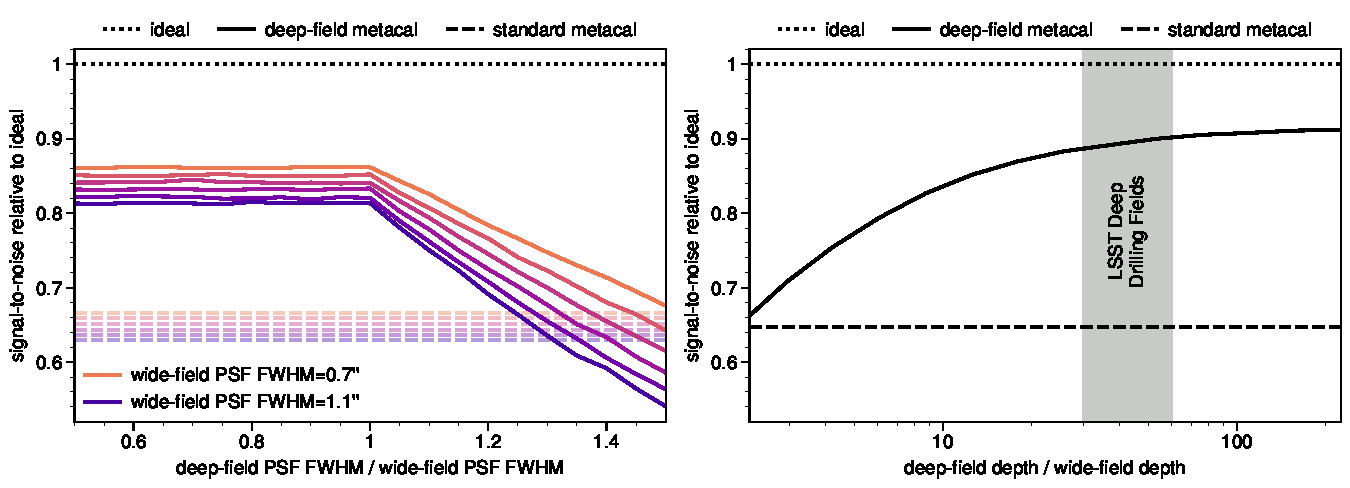
\includegraphics[width=\textwidth]{s2n_ratio.pdf}
    \caption{
      \textit{Left panel}: Signal-to-noise relative to ideal of sources processed deep-field and standard \mcal
      as a function of the ratio of deep-filed PSF FWHM to the wide-field FWHM. We assume the deep-field is
      10$\times$ deeper for this plot. The different colored solid lines show various wide-field PSF FWHMs ranging from 0.7'' to
      1.1'' for deep-field \mcal. The lower dashed lines of different colors show the result at the same wide-field PSF FWHM for
      standard \mcal. The dotted line is the ideal result of one.
      \textit{Right panel}: Signal-to-noise relative to ideal of sources processed with deep-field \mcal and standard \mcal as a function of the relative depth of the deep versus wide field. The FWHMs of the PSFs are fixed at 0.9''
      and 0.7'' for the wide and deep images. The solid line shows deep-filed \mcal and the lower dashed line shows standard \mcal.
      The dotted line is the ideal result of one.
      The solid gray band shows the estimated relative depth of the LSST Deep Drilling fields.
      Notice that in both the left and right panels, the maximum signal-to-noise for deep-field \mcal is limited to roughly 90\% of
      the ideal case. This effect is due to the increased size of the \mcal reconvolution PSF and our use of a fixed aperture moment
      for flux and shape measurement.}
    \label{fig:s2n}
\end{figure*}


\subsection{Effectiveness as a function of Relative PSF Size and Depth}\label{sec:sizedepth}

Now that we have established the accuracy of our technique, we turn our attention to the
expected gains in realistic survey scenarios where the relative sizes of the PSFs and
relative depths of the wide- and deep-field will vary. For this setup, we simulate
exponential galaxies with half light radii of 0.7'' with the wide-field PSF size varying
between 0.7'' and 1.1''. We take the deep-field to be a fixed $10\times$ deeper than the
wide-field and vary the ratio of the deep-field to wide-field PSF size from 0.5 to 1.5.
All PSFs are Gaussian. For each configuration, we measure the ideal signal-to-noise of
our galaxy, the signal- to-noise with standard \mcal, and the signal-to-noise with
deep-field \mcal.

The results of this test are shown in the left panel of Figure~\ref{fig:s2n}, where we
plot the signal-to-noise in units of the ideal signal-to-noise. The dashed horizontal
lines at the bottom of the figure show the results of standard \mcal. The colored
shading in the lines shows results for PSF FWHMs varying between 0.7'' and 1.1''. As
expected for the fixed, post-PSF aperture moments employed in this work, larger PSF
sizes reduce the overall signal-to-noise. The solid lines show the results of deep-field
\mcal. When the deep-field PSF is of the same size or smaller than the wide-field PSF,
we see substantial gains in the signal-to-noise. This gain matches our expectations from
the math above, $\sqrt{2/(1 + 2/10)}\approx1.3$, or about 30\% between the dashed and
solid lines on the left side of the plot. Notice however that even in the case where the
deep-field PSF is moderately larger than the wide- field PSF, deep-field \mcal is still
lower noise than standard \mcal.

The final salient feature of the plot is that even if deep-field \mcal is working its
best, we still find the signal-to-noise to be about $10\%$ lower than the ideal case,
shown as the dotted line. This feature is due to the increased size of the reconvolution
PSF used in the deep-field \mcal image manipulations. We have used a relatively
conservative setting of the reconvolution PSF size in this work. Better techniques to
set the reconvolution PSF size, like those employed in the Dark Energy Survey \mcal
shear measurements \citep{desy3shear} would result in smaller losses due to this effect.

Now we turn to the effects of the relative depth of the wide- and deep-field images. For
this test, we fix the sizes of the wide- and deep- field PSFs to 0.9'' and 0.7''
respectively and vary the depth of the deep-field image from 2$\times$ deeper to
$\sim200\times$ deeper than the wide-field image. We then again measure the
signal-to-noise in units of the ideal signal-to-noise for our test galaxy. The results
of this computation are shown in the right panel of Figure~\ref{fig:s2n}. The dashed
line in this panel shows the results of standard \mcal. The solid line shows the results
for deep-field \mcal. The dotted line shows the ideal result of one. We find, as
expected from the simple scaling
$\sqrt{\sigma^2_{\rm wide}/(\sigma^2_{\rm wide} + 2\sigma^2_{\rm deep})}$,
that as the depth of the deep-field image increases, our
technique becomes more effective. Again we see an overall loss of $\sim10\%$ in
signal-to-noise due to the reconvolution PSF. In the gray band, we show the estimated
relative depth of the LSST Deep Drilling Fields \citep[DDF,][]{lsst-ddf-depth}. While
the actual achieved depth of these fields is not known yet, for a broad range of
plausible depths, deep-field \mcal will be quite effective.

While the results of this section demonstrate the benefits of deep-field \mcal for
specific sources, the overall increase in the precision of a weak lensing analysis with
deep-field \mcal depends on the exact decreases in source shape noise and increases in
the effective number density due to the reduction in pixel noise. Further, for a survey
like the Rubin LSST, the exact area and depth the DDFs are not yet known. Similarly, we
do not yet know the relative PSF properties of the DDFs versus the main LSST survey. In
order to proceed, we make the following relatively conservative approximation. We assume
that the subset of the DDF images with the smallest PSF sizes are used to reach a depth
of only $10\times$ that of the main LSST survey. We then simulate objects as in case 4
above using the \descwl package assuming but assuming the DDFs and the main LSST survey
have the same PSF FWHM of 0.8''. We also fix the relative depth between the two and
neglect the PSF shape variations from case 4 to reduce noise in our estimate. For each
object, we measure its shear using standard \mcal and deep-field \mcal. We then compute
the error on the mean shear which is dictated by the same combination shape noise and
effective number density that enters the cosmic shear covariance matrix (i.e.
$\sqrt{\sigma_e^2/n}$ where $\sigma_e^2$ is the shape noise and $n$ is the number density
of sources). We find that deep-field \mcal achieves an $\approx15\%$ smaller
error on the mean shear relative to standard \mcal.  Note that
\citet{SheldonMcal2017} found that the increased pixel noise in standard
\mcal resulted in an resulted in a $\approx 20\%$ degradation in the precision of
statistical weak lensing measurements.  Our results thus suggest that the degradation
is reduced to a few percent with deep-field \mcal.  As our simulations do
not contain perfect realism, we conservatively estimate the degradation for deep-field
\mcal is $<5\%$.  In more realistic scenarios, we may be able to use more of the DDF
data resulting in better performance. We defer more detailed estimates to future work.

\subsection{Relative Importance of Different Correction Terms}\label{sec:terms}

In this section, we explore the relative importance of the two correction images,
Equations~\ref{eqn:cw} and \ref{eqn:cd}. We consider a setup like case 1 above, but we
remove one or both of these terms before computing the mean shear. For this case we also
match the PSFs of the wide- and deep-fields, keeping them both at 0.8''. We also use
sources with signal-to-noise of $\approx12$ to accentuate the effects of differing noise
on the shear calibration. We find that without the wide-field image correction term, the
shear recovery is biased with $m=47.5\pm8.7$ [$10^{-3}$ $3\sigma$ error]. Similarly
without the deep-field image correction term, we again find that the shear recovery is biased
with $m=-53.7\pm2.1$ [$10^{-3}$ $3\sigma$ error]. Finally without either term, we find
$m=-10.7\pm2.1$ [$10^{-3}$ $3\sigma$ error], indicating some degree of cancellation in
the various effects at play. The differing signs in the biases reflect changes in the
response to shear of the numerator of the deep-field \mcal estimator versus the
denominator. When removing the extra deep-field noise applied to the wide-field image
(i.e., Equation~\ref{eqn:cw}), the wide-field shape measurements respond more to shear
than the deep-field shape measurements, generating positive biases. Similarly, without
the extra wide-field noise applied to the deep-field image (i.e.,
Equation~\ref{eqn:cd}), the deep-field shape measurements respond more to shear than the
wide-field ones, generating negative biases. The two effects largely cancel, but leave
percent-level biases in the overall shear estimate indicating that to reach
high-precision, the noise distributions in the images must be treated carefully.


\begin{figure}
    \centering
    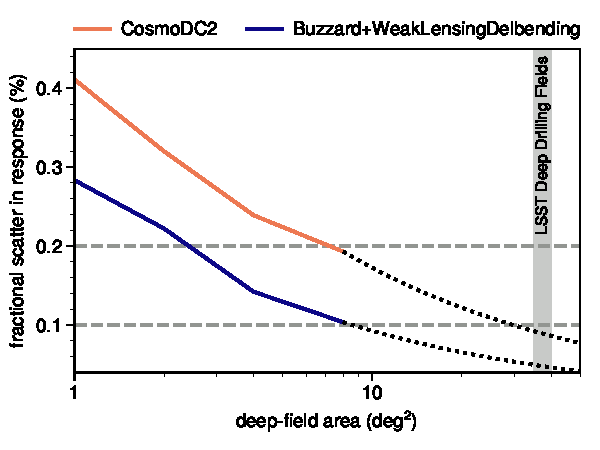
\includegraphics[width=0.45\textwidth]{sample_var.pdf}
    \caption{
      Sample variance scatter in the deep-field response as a function of the
      deep-field area. The different colored lines show the estimated sample variance
      from two different mock galaxy catalogs, \cosmodctwo and \buzzard+\descwl. The
      dashed lines represent the expected range of requirements on the shear
      calibration. The solid gray band shows the estimate area of LSST Deep Drilling
      Fields. The dotted lines show extrapolations to the LSST Deep Drilling Fields
      area assuming the sample variance scales as $1/\sqrt{\rm area}$. The LSST Deep
      Drilling fields will be large enough to result in sample variance scatter levels
      around 0.05\% to 0.1\%, meeting LSST requirements.
    }
    \label{fig:sample_variance}
\end{figure}


\subsection{Sample Variance}\label{sec:sv}

We now address the issue of sample variance in the deep-field dataset. The LSST DDF will
cover $\approx35$ deg$^2$ of area \citep{lsst-ddf-design,ivezic2019lsst}. In deep-field
\mcal, we compute the survey response only from the deep-field area. Thus sample
variance in the galaxy populations for this area will imprint itself in the \mcal
response, effectively increasing our final error on the multiplicative bias. This effect
is most easily characterized by the fractional scatter in the deep-field response
$\langle R_{d}\rangle$. This fractional scatter is directly comparable to our
requirements on the knowledge of the multiplicative bias $m$. For an LSST-like survey,
the final 10-year requirement will that the fractional scatter be less than 0.1\% to
0.2\% \citep{huterer2006,descsrd}.

In order to estimate the magnitude of this effect, we have used two different structure
formation models to compute the fractional scatter in the deep-field response as a
function of the deep-field area. The first is the \buzzard simulation set
\citep{derose2019buzzard} which uses the \textsc{ADDGALS} \citep{addgals} algorithm to
populate low-resolution N-body simulations with galaxies as a function of luminosity
and color. This method is able to provide $\approx5,000$ deg$^2$ of mock galaxy
populations. These catalogs match a variety of structure formation statistics at low
redshift, but their ability to make high-redshift predictions is not fully tested. The
\buzzard catalogs do not provide object shapes or sizes that correlate with large-scale
structure. To add in this effect, we use a simple matching technique, the basis of which
is described in \citet{galsampler}. We apply a linear transformation to the \buzzard
catalog to match the median and standard deviation of the $r-i$ and $i-z$ colors  of
objects in the \descwl catalog. To generate a specific deep-field data realization, we
first select a contiguous region of some area from the \buzzard catalog. We then find
the closest 100 galaxies from the \descwl catalog to each galaxy in the \buzzard catalog
in $r-i$-$i-z$ color-color space. We then select one of the 100 closest galaxies at
random, and use it in simulating our deep-field sample for this area. This process
imprints sample variance in the galaxy populations from \buzzard into the \descwl
catalog. The second model is the public \cosmodctwo \citep{cosmodc2} catalog. It
simulates a full set of galaxy properties in a 440 deg$^2$ area, including object shapes
and sizes that correlate with large-scale structure. This catalog has been used
extensively by the LSST Dark Energy Science Collaboration for simulating LSST-like
observations \citep{dc2,dc2note}.

For both models, we simulate the deep-field samples assuming the deep-field data is
10$\times$ deeper than the wide-field data. Due to the fact that the wide-field noise is
applied to the deep-fields, we cut the input simulation catalogs keeping only objects
brighter than $r$-band of $26$. For this specific test, we fix the PSF FWHM to 0.7'' for
both the wide- and deep-field images. With this setup, we compute the fractional scatter
in the shear response for a variety of assumed deep-field areas, ranging from 1 deg$^2$
to 8 deg$^2$. The results of this computation are shown in
Figure~\ref{fig:sample_variance}. We find that the fractional scatter decreases
approximately as $\sim1/\sqrt{\rm area}$ as one might expect. The simulations give
somewhat different results, with \cosmodctwo consistently about 0.1\% higher than the
\buzzard+\descwl model. For areas approaching that of the LSST DDF, we estimate a
residual fractional scatter in the range of 0.05\% to 0.1\% assuming a DDF area of 35
deg$^2$ and the $1/\sqrt{\rm area}$ scaling. This level of sample variance will meet or
exceed LSST requirements.

We have examined the galaxy properties of the \cosmodctwo and \buzzard+\descwl samples
in order to understand why they give different results. We find that the \cosmodctwo
model has a broader variance in the bulge-to-disk ratio while the shape noise
distributions are largely similar. We also find that the \cosmodctwo catalog has a
slightly higher number density of objects, with $\approx65\ {\rm objects}/{\rm
arcmin}^2$ as opposed to the \buzzard+\descwl catalogs with only $\approx50\ {\rm
objects}/{\rm arcmin}^2$. This difference in number density does not account for the
differences in the response sample variance scatter. Regardless of the exact nature of
the differences between the catalogs, our current results indicate that for a broad
range of assumptions about the LSST DDF samples, deep-field \mcal will be an effective
technique.


\section{Summary}\label{sec:conc}

In this work, we have developed a new technique called deep-field \mcal. It allows one
to combine images from deep- and wide-field data sets to measure weak lensing
gravitational shear using \mcal-type methods but at higher precision. In particular our main
conclusions are:
\begin{itemize}
  \item Deep-field \mcal allows one to combine images from wide- and deep-field surveys
    to measure \mcal weak lensing shears at below part-per-thousand accuracy
    (Section~\ref{sec:mc}, Table~\ref{tab:shearmeas}) while reducing the pixel noise
    in \mcal images by $\approx30\%$ (Section~\ref{sec:sizedepth}).
  \item The exact decrease in pixel noise depends on the details of
    the wide- and deep-field depth and PSF distributions (Section~\ref{sec:sizedepth}).
  \item When applied to the Rubin LSST, we expect an at least $\approx15\%$ increase in
    the precision of weak lensing analyses due to the decreased pixel noise contributions
    to the shape noise and increased effective source density.  We conservatively
    estimate that the corresponding degradation in the precision of statistical
    shear measurements is reduced from 20\% for \mcal to $<5\%$ for deep-field \mcal.
  \item The LSST DDFs will have enough area to suppress the effects of sample variance
    in the deep-fields to levels that will meet LSST requirements
    (Section~\ref{sec:sv}).
  \item Deep-field \mcal will extend naturally to \mdet due to the fact that it
    explicitly matches the PSF of the deep- and wide-field images, ensuring detection
    and blending biases are properly calibrated (Section~\ref{sec:deepmcal}).
\end{itemize}

We have also discussed several avenues for improving the algorithms presented in this
work. These include relaxing the PSF matching requirement (Section~\ref{sec:deepmcal}),
optimizing how one pairs the wide- and deep-field images in order to reduce
signal-to-noise losses from PSF matching (Section~\ref{sec:statmatch}), reducing
computing costs through reducing duplication in the deep-field precessing
(Section~\ref{sec:statmatch}), and reducing sample variance in the deep-field response
computations through reweighting the deep-field catalogs within \mcal/\mdet to better
match the wide-field object distributions (Section~\ref{sec:statmatch}).

Another important avenue of further research is attempting to use the algorithms
presented in this work to inject sheared synthetic sources in image postage stamps into
existing survey images. Shear measurements made in images with these injected sources
can potentially help constrain cross-redshift response biases in weak lensing shape
measurements \citep{desy3imsims}. At a technical level, one requires that shape
measurements of the injected sources be unbiased when those sources are isolated. The
techniques presented in this work show how to match the PSF and noise distributions of
sheared deep-field and unsheared wide-field images, a necessary prerequisite for
statistically correct injections.

Finally, it is important that this work be extended to test deep-field \mdet directly.
While we are confident in the overall idea, there may be unforeseen issues related to
handling real-world effects like image coaddition, masking/artifacts, bright stars, etc.
Detailed tests of deep-field \mdet will be needed to ensure our techniques can reach
their full potential.

In the future, we plan to pursue the improvements above, explicit tests of deep-field
\mdet for LSST-like surveys, and the application of deep-field \mdet to Rubin LSST data.
The techniques presented in this work are promising but require detailed and systematic
testing in order to be fully ready for next-generation weak lensing surveys.

\section*{Acknowledgments}

MRB is supported by DOE grant DE-AC02-06CH11357. We thank Joe DeRose and Risa Wechsler
for providing the \buzzard simulation used in this work. We thank the \cosmodctwo team
for publicly releasing their mock galaxy catalogs. We thank Andrew Hearin and Eduardo
Rozo for extremely helpful comments that greatly improved the presentation of this work.
We gratefully acknowledge the computing resources provided on Bebop, a high-performance
computing cluster operated by the Laboratory Computing Resource Center at Argonne
National Laboratory, and the RHIC Atlas Computing Facility, operated by Brookhaven
National Laboratory. This work also used resources made available on the Phoenix
cluster, a joint data-intensive computing project between the High Energy Physics
Division and the Computing, Environment, and Life Sciences (CELS) Directorate at Argonne
National Laboratory. This work made extensive use of the Astrophysics Data Service (ADS)
and \texttt{arXiv} preprint repository. We thank the maintainers of the
\texttt{GCRCatalogs}, \citep{gcrcatalogs}, \texttt{numpy} \citep{numpy}, \texttt{scipy}
\citep{scipy}, \texttt{numba} \citep{numba}, \texttt{Matplotlib} \citep{matplotlib}, and
\texttt{conda-forge} \citep{condaforge} projects for their excellent open-source
software and software distribution systems.

\bibliographystyle{aasjournal}
\bibliography{references}

% \appendix

\end{document}
